
\section{Data Preparation}

\subsection{Data Cleaning}

The dataset was systematically inspected for quality issues before any modeling. Each cleaning step was performed explicitly and its result documented to ensure full transparency.

\begin{table}[H]
\centering
\caption{Data cleaning summary}
\begin{tabular}{lll}
\toprule
\textbf{Check} & \textbf{Finding} & \textbf{Action Taken} \\
\midrule
Missing values & 0 across all 61 columns & No imputation needed \\
Duplicate rows & 0 duplicates found & No removal needed \\
Non-numeric columns & \texttt{url} (string) & Dropped (non-predictive) \\
Non-predictive columns & \texttt{url}, \texttt{timedelta} & Dropped (2 columns removed) \\
Data types & All 59 remaining columns numeric & No encoding needed \\
Binary indicators & 13 columns (weekday, channel flags) & Used as-is \\
Outliers (\texttt{shares}) & IQR method: 10,072 outliers (25.4\%) & \textbf{Not removed} (see below) \\
\bottomrule
\end{tabular}
\end{table}

\noindent The target variable \texttt{shares} showed a strongly right-skewed distribution (min: 1, max: 843,300, median: 1,400). Using the IQR method, 25.4\% of articles were flagged as outliers. These outliers were \textbf{not removed} because they reflect the natural behavior of online engagement, where a small number of articles can become highly viral. Instead, the skewness was handled during regression tasks using the transformation $\log(1 + \texttt{shares})$, which stabilizes the variance while preserving the data structure.

After cleaning, the working dataset contained \textbf{39,644 rows} and \textbf{59 numeric columns} (58 features + 1 target).

\subsection{Preprocessing: Before vs.\ After}
\label{sec:preprocessing_definition}

To study the impact of preprocessing on model performance, all supervised tasks (Tasks~1, 2, 5, and 6) were evaluated under two conditions:

\begin{itemize}[leftmargin=1.5em]
    \item \textbf{Before Preprocessing (Raw):} Features were imputed using median values (via \texttt{SimpleImputer}) but \textit{not scaled}. This tests how models perform on the original feature magnitudes.
    \item \textbf{After Preprocessing (Processed):} Features were imputed with medians and then standardized using \texttt{StandardScaler} (zero mean, unit variance). This benefits scale-sensitive models such as Logistic Regression, KNN, and SVM.
\end{itemize}

\noindent Both conditions used the same train/test split (80/20, stratified for classification, random seed = 42) to ensure a fair comparison.

\subsection{Exploratory Data Analysis}
Exploratory Data Analysis (EDA) was conducted to understand the overall behavior of the dataset before feature engineering and model training, following standard data mining practice \cite{han2011datamining,bishop2006prml}.

The distribution of \texttt{shares} was found to be heavily right-skewed, with most articles receiving relatively modest engagement and a much smaller number receiving extremely high shares. This observation justified the use of log transformation in the regression setting.

\begin{figure}[H]
    \centering
    
\includegraphics[width=0.75\textwidth]{figures/fig1_hist_shares.png}
    \caption{Histogram of article shares showing the strong right-skewed distribution of the target variable.}
    \label{fig:hist_shares}
\end{figure}

\begin{figure}[H]
    \centering
    
\includegraphics[width=0.55\textwidth]{figures/fig2_boxplot_shares.png}
    \caption{Boxplot of article shares highlighting the presence of many extreme outliers.}
    \label{fig:boxplot_shares}
\end{figure}

Correlation analysis showed moderate to strong relationships among some groups of features, especially within keyword-related variables and certain self-reference statistics. This suggested the presence of redundancy in the original feature space and motivated the need for feature selection.

\begin{figure}[H]
    \centering
    
\includegraphics[width=0.82\textwidth]{figures/fig3_correlation_heatmap.png}
    \caption{Correlation heatmap of selected numerical features before feature selection.}
    \label{fig:corr_heatmap_before}
\end{figure}

Additional descriptive analysis indicated that articles published on weekends tend to receive somewhat higher engagement on average than those published on weekdays. This observation later informed the association rule and publication timing tasks.

\begin{figure}[H]
    \centering
    
\includegraphics[width=0.72\textwidth]{figures/fig4_scatter_plot.png}
    \caption{Scatter plot showing the relationship between article length and number of shares.}
    \label{fig:scatter_tokens_shares}
\end{figure}

\begin{figure}[H]
    \centering
    
\includegraphics[width=0.7\textwidth]{figures/fig5_bar_chart.png}
    \caption{Average shares by publication day, showing slightly stronger engagement on weekends.}
    \label{fig:weekday_bar}
\end{figure}

\begin{figure}[H]
    \centering
    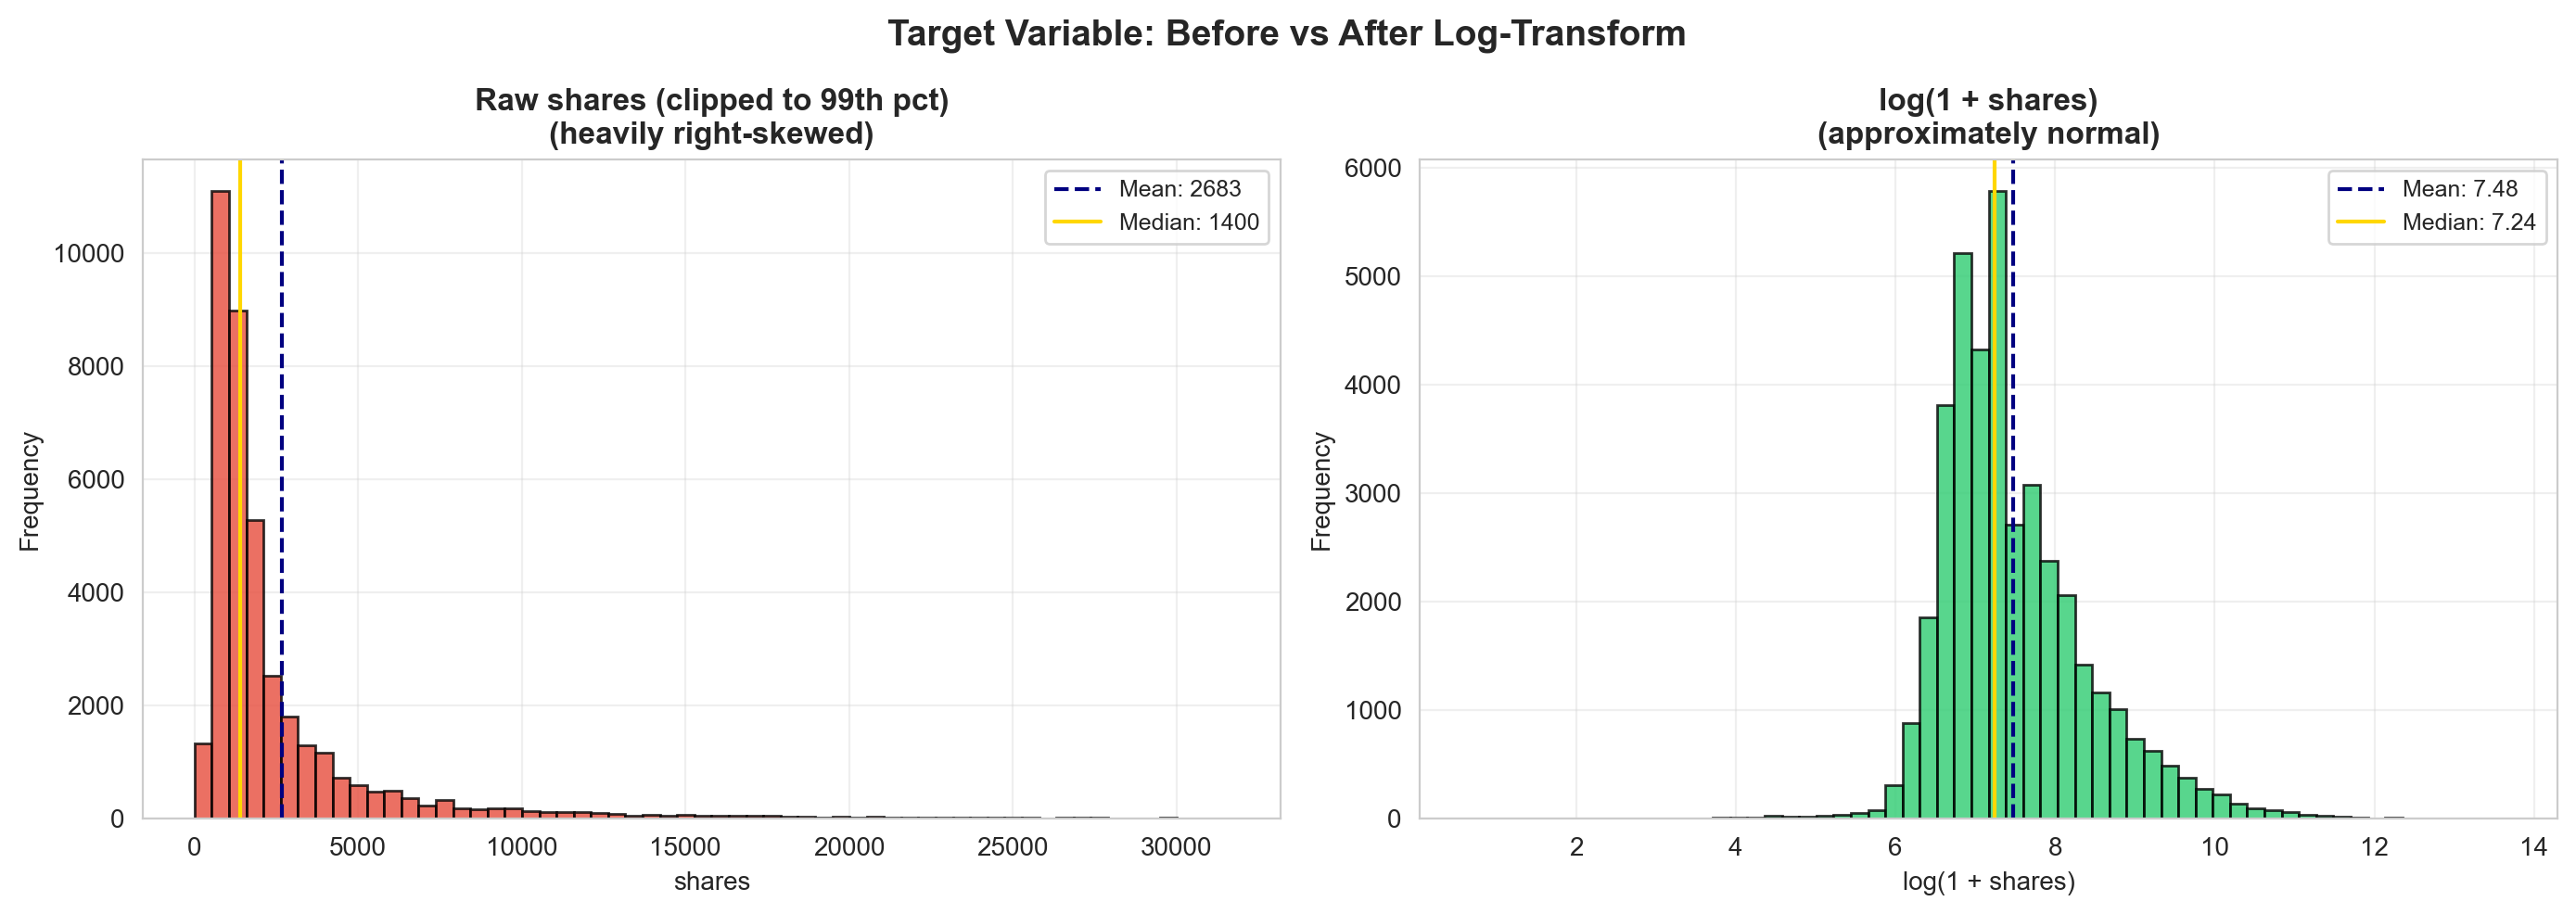
\includegraphics[width=0.9\textwidth]{figures/exp_fig1_shares_vs_log_shares.png}
    \caption{Comparison of the raw \texttt{shares} distribution and the log-transformed target used in regression tasks.}
    \label{fig:shares_vs_logshares}
\end{figure}

Overall, the EDA stage helped identify three key properties of the dataset: skewness in the target variable, redundancy among some predictors, and mild temporal variation in engagement. These findings guided the feature engineering and modeling choices used in later sections.
